\chapter{Player Skills}
\label{Agent}

In this chapter we are going to present the main functions that are necessary for the agent to be functional in the field. Every part of the agent's software and supported player skills will be extensively described below. 


\section{Agent Architecture}
\label{Architecture}

Before examining each individual skill of our players, it is important to describe the general architecture of our agents, which is shown in  Figure~\ref{fig:Architecture}. The Soccer Simulation Server (\textit{rcssserver3d}) is responsible for communicating perceptor messages to the agent. The Connection component handles this connection between the agent and the server. These messages are handled by a string parser, which stores the incoming observations in various data structures. Consequently, the functions that require these new observations  to update the agent's Beliefs are now ready to proceed. Self-localization of the agent into the field or a check if the agent has fallen on the ground are few of those belief updates. Behavior is a major component of any agent. The agent has to combine all the available knowledge and beliefs about the world state and act properly. Behavior is the function which takes as input argument the agent's beliefs about the world state and computes an action to be executed by the agent as output. The Coordination component is responsible for assigning roles to different agents implementing the strategy of team. Communication  and Motion are responsible for handling agent's requests for sending messages to teammates and executing movements respectively. These two components send effector messages to the Connection component in each cycle, if necessary, and these messages are relayed to the soccer simulation server.

\begin{figure}[t!]
\centering
  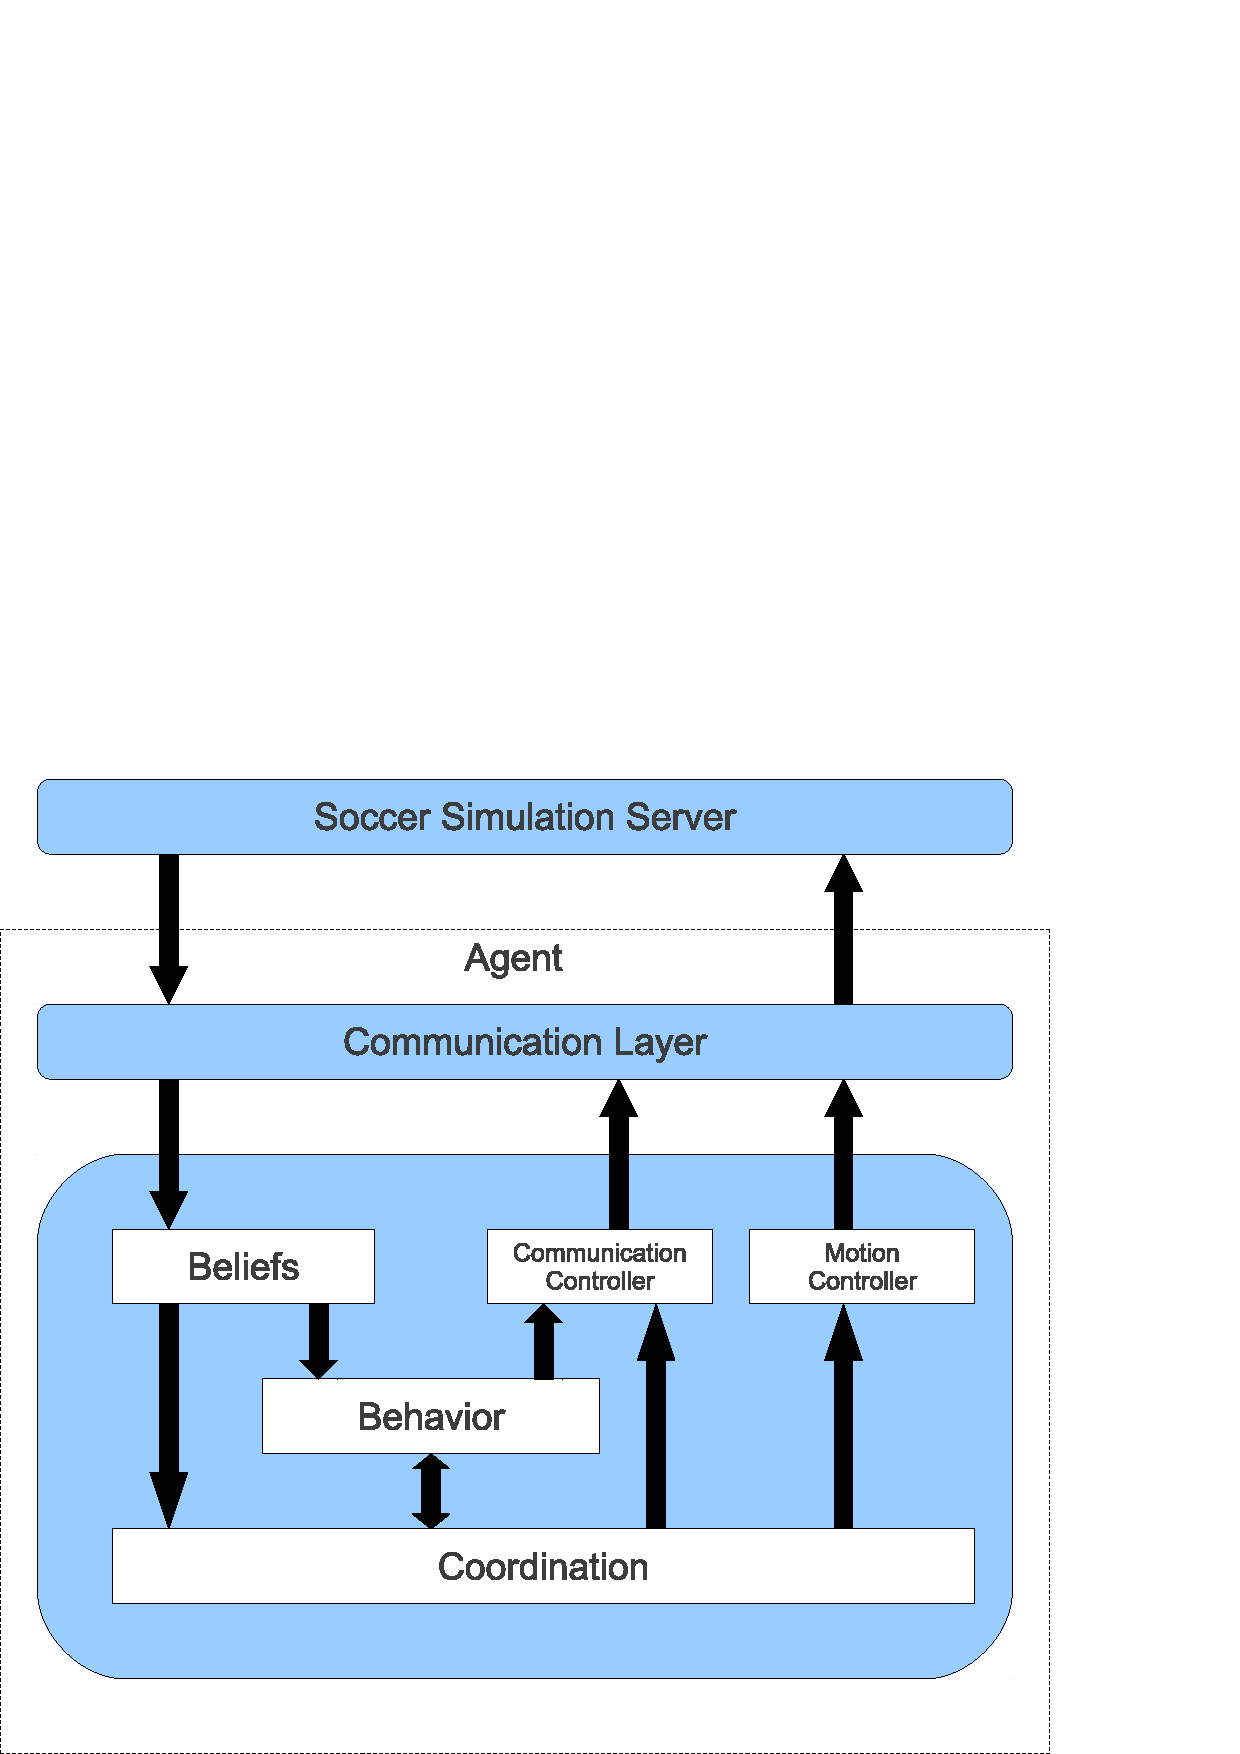
\includegraphics[width=0.8\textwidth]{Chapter3/figures/Arch.pdf}
  \caption{The Agent Architecture.}
  \label{fig:Architecture}
\end{figure}


\section{Connection}
The SimSpark server hosts the simulation process that manages the soccer simulation. It is responsible for advancing the game from each cycle to the next. So, it is obligatory for each agent to be connected to the server at all times during a simulated game. Agents receive sense messages from the server every 20ms at the beginning of each simulation cycle; these messages include information about all agent's perceptions. Agents willing to send action messages, can do so at the end of their think cycles, which may or may not coincide with the simulation cycles. If these two cycles coincide, the server is going to receive the action message at the same time it sends the next sense message. Figure~\ref{fig:Simulation-Update-Loop} shows how the communication between server and agent takes place over consecutive cycles.

\begin{figure}[t!]
\centering
  \includegraphics[width=0.8\textwidth]{Chapter3/figures/SimulationUpdateLoopSynchronizationBetweenSimSparkAndAgent.png}
  \caption{Server and Agent Communication.}
  \label{fig:Simulation-Update-Loop}
\end{figure}

%testchange for git

\section{Perceptions}
Perceptions in simulated soccer are quite different compared to those in  real soccer games. Agents do not have to process raw data coming directly from sensors, but rather listen to sensor and higher-level observation messages sent by the server at each cycle. These messages take the following form:

\begin{verbatim}
(time (now 46.20))(GS (t 0.00) (pm BeforeKickOff))(GYR (n torso)
(rt 0.00 0.00 0.00))(ACC (n torso) (a 0.00 -0.00 9.81))(HJ (n hj
1)(ax 0.00))(HJ (n hj2) (ax 0.01))(See (G2R (pol 14.83 -11.81 1.
08))(G1R (pol 14.54 -3.66 1.12)) (F1R (pol 15.36 19.12 -1.91))(F
2R (pol 17.07 -31.86 -1.83)) (B (pol 4.51 -26.40 -6.15)) (P (tea
m AST_3D)(id 8)(rlowerarm (pol 0.18 -35.78 -21.65)) (llowerarm (
pol 0.19 34.94-21.49)))(L (pol 8.01 -60.03 -3.87) (pol 6.42 51.1
90 -39.13 -5.17))(L (pol 5.91 -39.06 -5.11) (pol 6.28-29.26 -4.8
8)) (L (pol 6.28 29.34 -4.95)(pol 6.16 -19.05 -5.00)))(HJ(n raj1
) (ax -0.01))(HJ (n raj2) (ax -0.00))(HJ (n raj3)(ax -0.00))(HJ(
n raj4) (ax 0.00))(HJ (n laj1) (ax 0.01))(HJ (n laj2) (ax 0.00)) ...\end{verbatim}

\noindent
The above message is an example message our agent may receive from the server during simulation. It includes information about the server time, the game state and time, values for each one of the joints, visual observations from the camera, and data from the accelerometer, gyroscope, and force sensors. We parse these messages and save the enclosed information in data structures appropriate for each type of perception. 

%Figure~\ref{fig:BeliefsUpdate} illustrates this procedure.
%\begin{figure}[t!]
%\centering
%  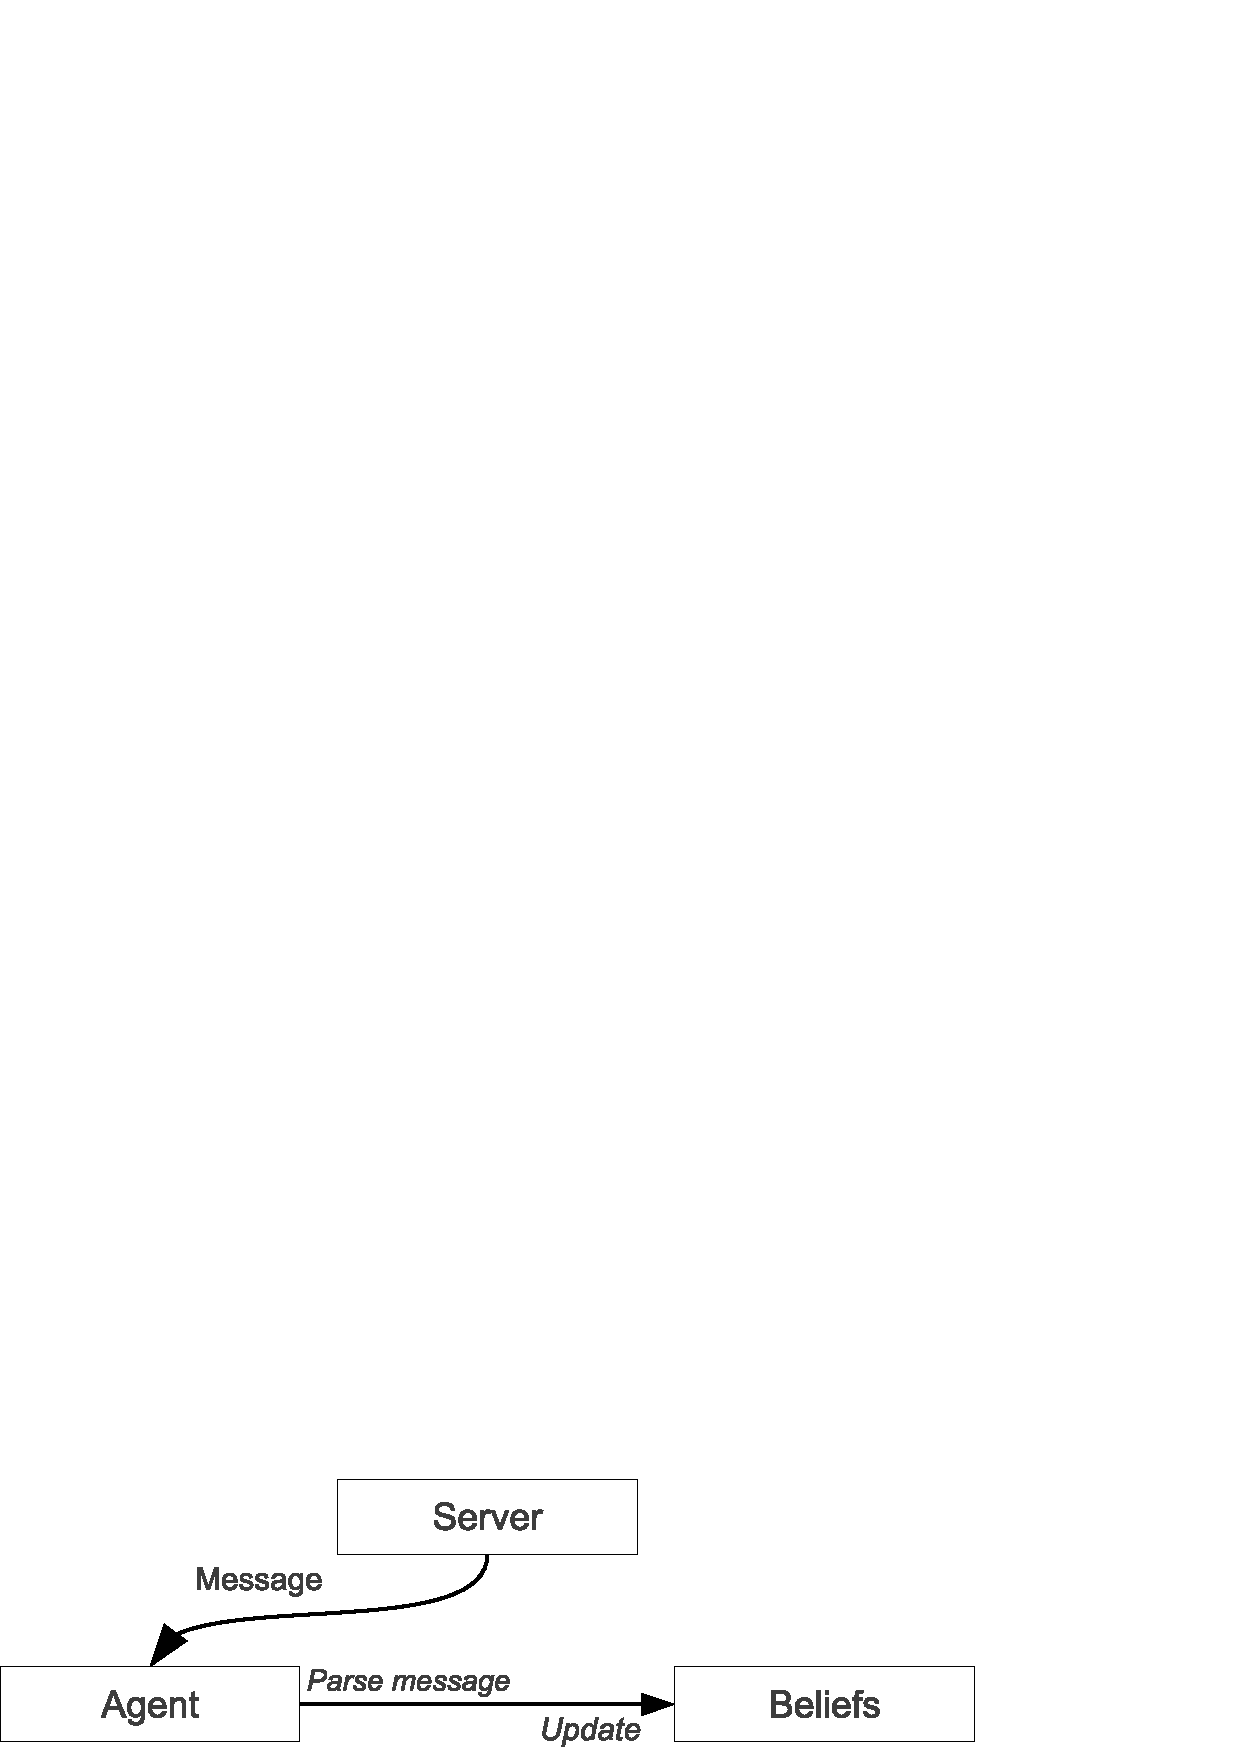
\includegraphics[width=0.8\textwidth]{Chapter3/figures/Message.pdf}
%  \caption{Beliefs Update.} 
%  \label{fig:BeliefsUpdate}
%\end{figure}


\section{Localization}
Once we have all the new perceptions from the server available, we can update our agents' belief about its current self-location in the field and the current location of other objects of interest (ball, teammates, opponents). Our localization scheme is largely based on a method proposed by a colleague within a common course project~\cite{Localization}. Localization, as a process, is executed every three cycles (60ms), in fact every time we receive observations from the vision perceptor. 
A key restrictive factor is that the agents are equipped with a restricted vision perceptor which limits the field of their view to 120 degrees. 
%An example of this limitation is shown in Figure~\ref{fig:fieldofview}. 
It is easy to realize that the localization process would have been easier, if there was an omni-directional vision perceptor.





\subsection{Self Localization} 

The potentially visible objects in our current field of view may be of different types: ball, landmarks, teammates, and opponents. After registering all currently visible objects, we first use only the landmarks, which are located at permanent known positions in the field, to derive candidate self-locations and update the agent's belief about the current position and orientation in the field. There are eight landmarks in the field, shown in Figure~\ref{fig:fieldofview}: the four field corners (F1R, F2R, F1L, F2L) and the goalposts of the two goals (G1R, G2R, G1L, G2L). These eight landmarks cannot be all visible simultaneously at the same time; in general, the number of visible landmarks at any time for a player located within the field will range from zero to four. For example, given the current location of the agent in Figure~\ref{fig:fieldofview}, there are only three visible landmarks: F1R, G1R, G2R. 

\begin{figure}[t!]
\centering
  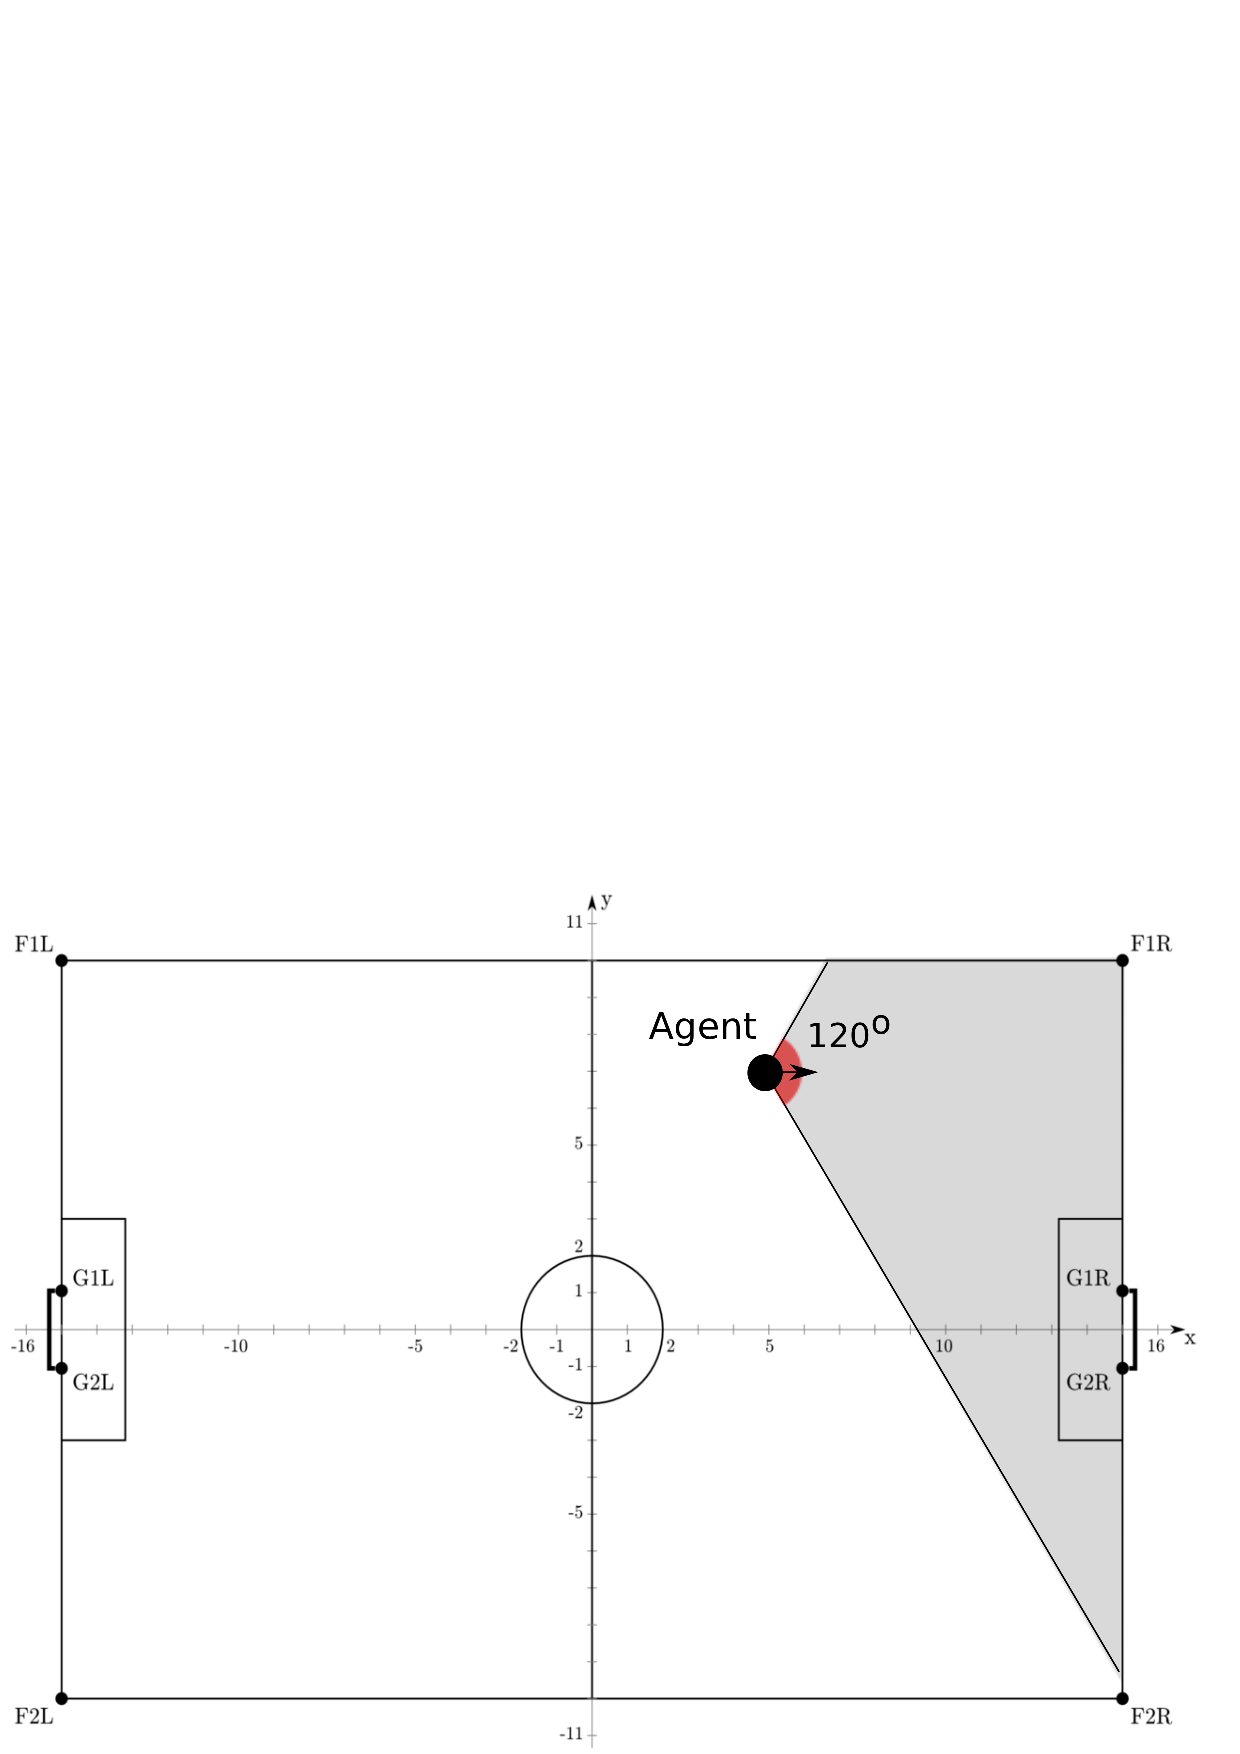
\includegraphics[width=0.8\textwidth]{Chapter3/figures/LViewAngle.pdf}
  \caption{Nao's Restricted Field of View and Field Landmarks.} 
  \label{fig:fieldofview}
\end{figure}

The self-localization function takes the distance, as well as the horizontal and vertical angles of two currently visible landmarks as input and returns a candidate self location $(x,y,\theta)$ as output, where $(x,y)$ are the coordinates in the field and $\theta$ is the orientation of the body with respect to the angle system of the field. The two visible landmarks form two circles with radius equal to the observed distance to each one of them centered at the static and known coordinates of these landmarks. Obviously, these two circles intersect at two points, which represent two candidate self locations. We reject the wrong candidate using the horizontal viewing angles of the two landmarks and also the fact that the correct candidate cannot be way outside the field. Figure~\ref{fig:Localization} shows a typical example of self localization with two landmarks. In cases where the agent sees more than two landmarks, the self-localization function is called for each pair of landmarks. The final estimated location is computed as the average of the outcomes of all pairs. Apparently, when the agent has less than two visible landmarks in the current field of view, the self-localization update does not take place.   

\begin{figure}[t!]
\centering
  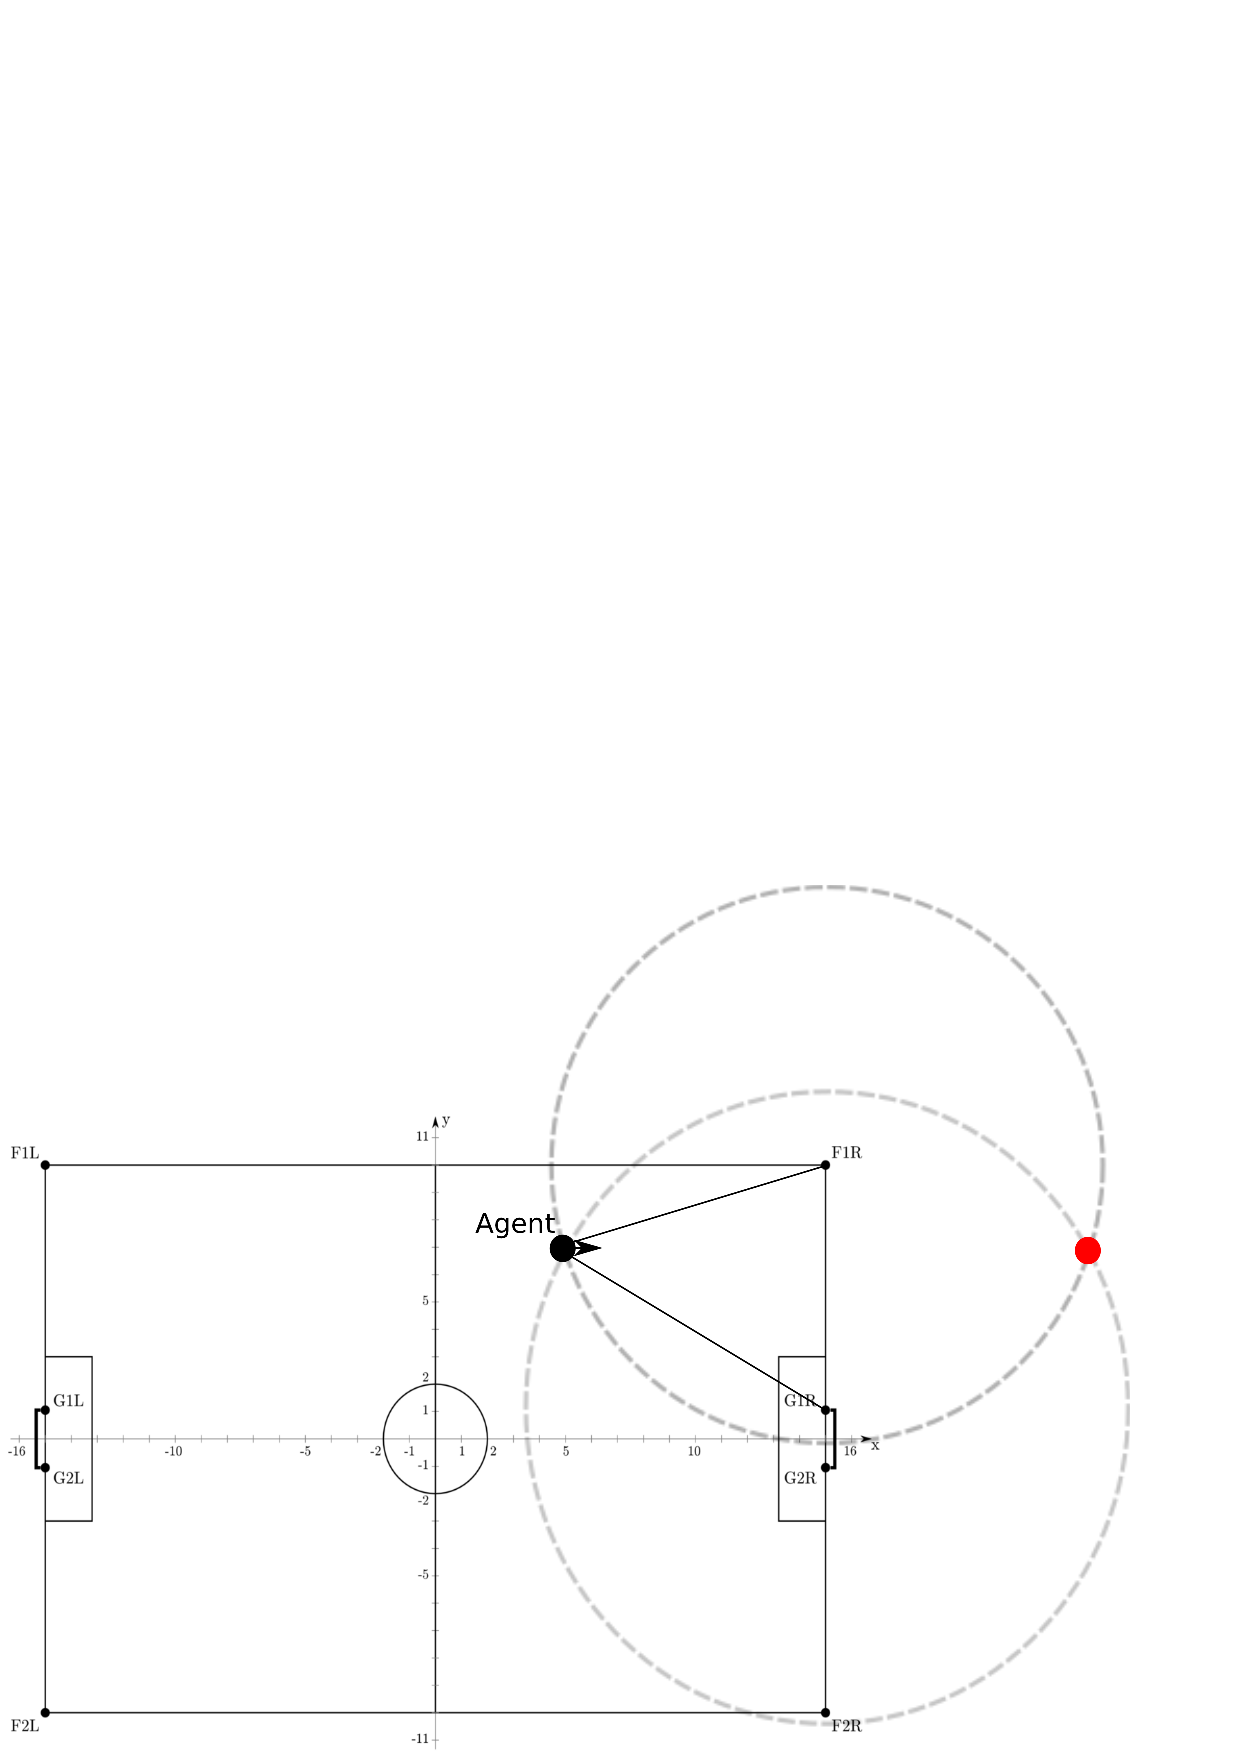
\includegraphics[width=0.8\textwidth]{Chapter3/figures/Localization.pdf}
  \caption{Self-Localization Example with the F1R and G1R Landmarks.} 
  \label{fig:Localization}
\end{figure}

\subsection{Object Localization} 

Apart from self localization, it is important to be able to compute the position of other visible objects, such as opponents and the ball (note that there is no need to localize teammates in the field; their beliefs are shared via communication). Knowing our own location in the field helps us locate other visible objects too. For each currently visible object, the vision perceptor informs us about its vertical and horizontal angles and its distance from the agent. This information is sufficient for the calculation of their exact positions into the field's coordinate system. Figure~\ref{fig:LocalizationResults} shows an example scenario of calculating the positions of the ball and an opponent. To successfully locate other objects in the field, the same condition as in self localization applies: there must be at least two visible landmarks. If the currently visible landmarks are less than two, other objects cannot be located in the field using the current perceptions; nevertheless, the agent knows where they are located with respect to itself. 



\begin{figure}[t!]
\centering
  \includegraphics[width=0.8\textwidth]{Chapter3/figures/LocalizationResults.pdf}
  \caption{Object (Ball and Opponent) Localization Example.} 
  \label{fig:LocalizationResults}
\end{figure}
\hfill





\subsection{Localization Filtering}
In the absence of a more sophisticated probabilistic localization scheme, we are forced to ensure that localization results are qualitative enough for us to rely on. Due to the temporary misses of landmarks from the field of view and the noisy observations from the vision perceptor, localization based only on the current perception is not always accurate enough to depend upon. Therefore, a simple filtering procedure on estimates computed by the localization process is employed to update the agent's belief about self locations and positions of other objects over time. 


\begin{algorithm}[ht!]
\caption{Localization Filtering}
\label{LocalizationFiltering}
\begin{algorithmic}[1]
\STATE {\bf Input: }$LastEstimate$
\STATE {\bf Output: }$FilteredLocation$
\STATE $Queue$: a FIFO queue storing the $MaxSize$ (default=10) most recent estimates
\STATE 
\IF{$size(Queue) = 0$}
\STATE $Queue.Add(LastEstimate)$
\ELSIF{$LastEstimate \not\approx AverageLocation(Queue)$}
\STATE $Queue.Remove()$
\ELSE 
\IF{$size(Queue) = MaxSize$}
\STATE $Queue.Remove()$
\ENDIF
\STATE $Queue.Add(LastEstimate)$
\ENDIF
\RETURN $AverageLocation(Queue)$
\end{algorithmic}
\end{algorithm}

 
In general, the localization process provides the agent with numerous estimated locations over time. The general idea we adopt is based on the fact that these estimates do not include long sequences of consecutive faulty estimates. Therefore, it is fairly easy to ignore sporadic faulty estimates (outliers), while updating the agent's belief.
To address this problem, we came up with a simple localization filtering algorithm outlined in Algorithm~\ref{LocalizationFiltering}. We maintain a FIFO queue which stores the most recent non-faulty location estimates. The average of the locations in the queue consist the agent's belief about its location in the field at any time. When a new estimated location arrives from the localization process, we first check if the queue is empty; in this case, we simply insert this estimate into the queue. Otherwise, we check if the newly arrived estimate ``agrees'' with the current belief, whereby ``agrees'' means that they are not far apart. If not, this estimate is ignored and additionally one element of the queue is removed. This step represents a simple way of discounting the current belief in the presence of an outlier estimate. If the outlier estimate corresponds to a correct location, it will persist, eventually it will discard the entire queue with the current belief, and afterwards it will initiate a new belief in the empty queue. Finally, if the new estimate ``agrees'' with the current belief, it is inserted in the queue to reinforce the current belief, replacing one element (the oldest one), if the queue has reached capacity. This simple filtering scheme smooths out the belief of our agent's location and rejects most faulty estimates.

Localization filtering applies both to the calculation of the agent's self location and to the calculation of the ball's position. For the sake of efficiency, we do not use it to filter opponent positions. As mentioned already, the filtered locations of teammates are shared among team members via communication. The end effect of localization filtering is a significant improvement on the localization outcome, so that we can rely upon it with confidence. 



\section{Motion}
\label{Motions}

\begin{figure}[t!]
\centering
  \includegraphics[width=0.4\textwidth]{Chapter3/figures/Models_NaoAnatomy.png}
  \caption{Nao's anatomy: kinematic chains and joints.}
  \label{fig:NaoAnatomy}
\end{figure}

The simulated Nao robot comes with 22 degrees of freedom, corresponding to 22 hinge joints. Figure~\ref{fig:NaoAnatomy} shows Nao's anatomy with all joints, split in five kinematic chains (head, left arm, right arm, left leg, right leg).
In robotics, a complex motion is commonly defined as a sequence of timed joint poses. A pose is a set of values for every joint in the robot's body or in a specific kinematic chain at a given time. 
For any given set of $n$ joints a pose at time $t$ is defined as:
\[
Pose(t)= \lbrace J_{1}(t), J_{2}(t), \ldots ,J_{n}(t) \rbrace
\]
Motion is an important part of every team participating into the RoboCup 3D Simulation League. Motions can be static or dynamic. Most teams in this league make use of dynamic motions, which give a major advantage on their side, at the expense of complexity. In our work, we are using predefined static motion files. Motion files describe timed sequences of poses, which provide fixed values for each joint at specific times; when executed, these sequences achieve some kind of desired motion. The difference between static motion files and dynamic motion is that the latter makes use of forward and inverse kinematics, as well as calculation of the center of the robot's body mass, to derive sequences of poses dynamically. These dynamically computed motions can be corrected on the fly for better body balance and faster movement. Since our goal was to study coordination algorithms, we chose to work with the simpler approach of static, yet effective, motion files with some dynamic enhancements. In our approach, we are using two kinds of such files: XML-based and text-based.


\subsection{XML-Based Motion Files}
These motion files have been created and distributed by FIIT RoboCup 3D project~\cite{fiit} and they provide forward walk, left and right side steps, strong and regular kicks, stand-up, and left and right goalkeeper fall motions. These files have an intuitive XML structure, which facilitates integration into our project. The general structure of these XML-based motion files is shown below.
\begin{verbatim}
<phase name="Start" next="Phase1">
   <effectors>
      Joint Values
   </effectors>
   <duration>duration</duration>
</phase>

<phase name="Phase1" next="Phase2">
   <effectors>
      Joint Values
   </effectors>
   <duration>duration</duration>
</phase>

<phase name="Phase2" next="Phase1">
   <effectors>
      Joint Values
   </effectors>
   <duration>duration</duration>
   <finalize>Final</finalize>
</phase>

<phase name="Final">
   <effectors>
      Joint Values
   </effectors>
   <duration>duration</duration>
</phase>
\end{verbatim}
As shown in the structure of this XML file, each movement is split into phases. Each phase has a duration and values for every joint of the robot or the kinematic chain(s) related to the movement. Moreover, each phase has an index which points to the next phase. For example, the first phase (\texttt{Start}) has an index to the next phase (\texttt{Phase1}). Phases with a \texttt{finalize} field can be used to end the corresponding movement. For example, phase \texttt{Phase2} has a finalize index which points to phase \texttt{Final}; this means that, if we want to end the execution of this movement, we have to do it in phase \texttt{Phase2} by transitioning to phase \texttt{Final} instead of continuing with the next phase (\texttt{Phase1}).

\subsection{XML-Based Motion Controller}

The motion controller is a major component in our software which enables and controls the movement abilities of the robot. It is responsible for handling the movement requests of the agent. Agents do not have direct access to robot joints and joint poses, but can trigger desired motions by posting requests to the motion controller in the form of values to a specific variable. Each agent declares in this variable the movement he is willing to perform. In each cycle, the motion controller reads this variable and generates an appropriate hinge joint effector string, aiming at either terminating a running motion request (if different than the new one), or initiating the requested one (if there was no running request), or simply continuing with the execution of the current request (if initiated earlier). In effect, the motion controller satisfies a motion request posted by the agent, even if the completion of the motion takes several cycles, ensuring that transitions between different motions are smooth. 


\begin{figure}[t!]
\centering
  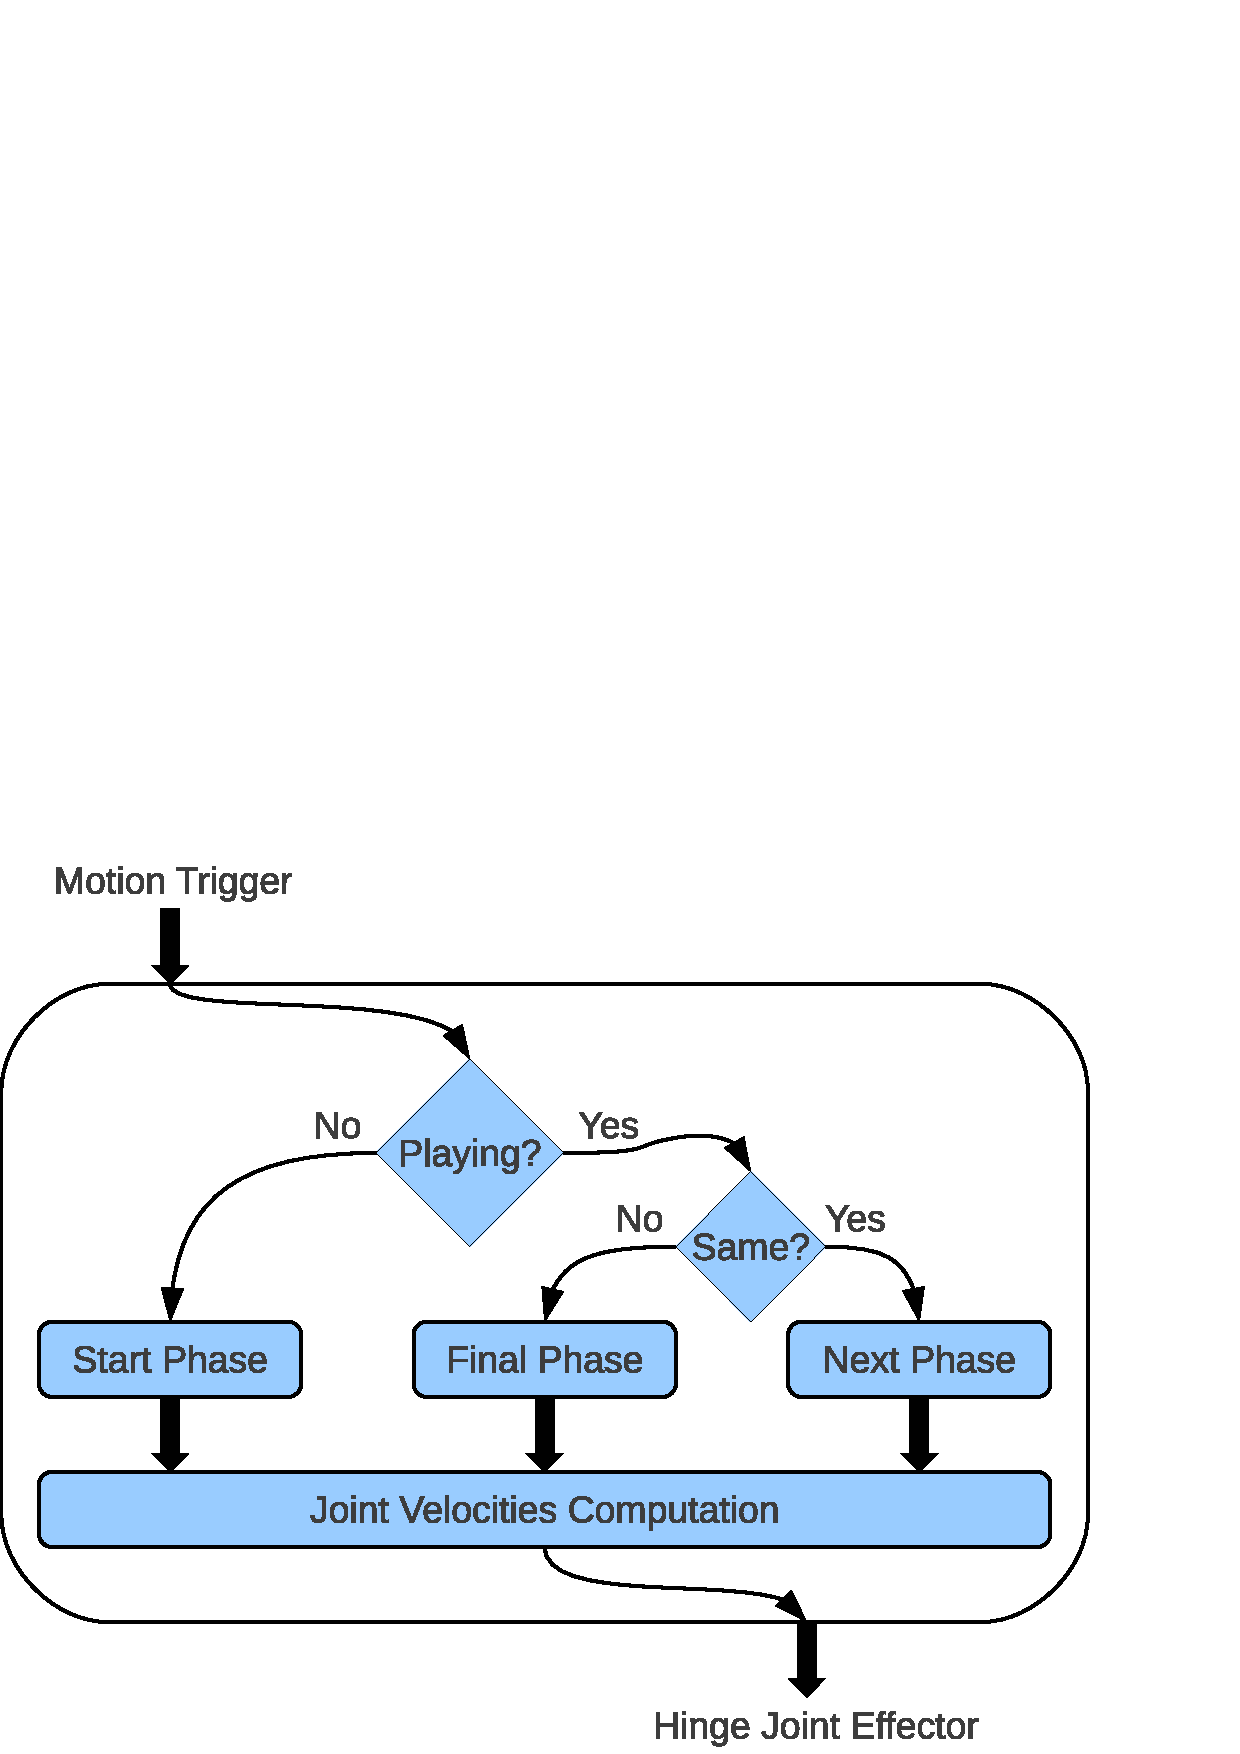
\includegraphics[width=0.6\textwidth]{Chapter3/figures/MotionController.pdf}
  \caption{XML-Based Motion Controller.}
  \label{fig:MotionController}
\end{figure}


Figure~\ref{fig:MotionController} describes the general architecture of the XML-based motion controller. The motion controller checks if there is a motion which is playing already. If the currently playing motion is the same as the requested one, the motion controller continues with the next of its phases; if not, the controller tries to finalize the playing movement in order to start playing the newly requested one (in a future cycle).


\begin{figure}[t!]
\centering
  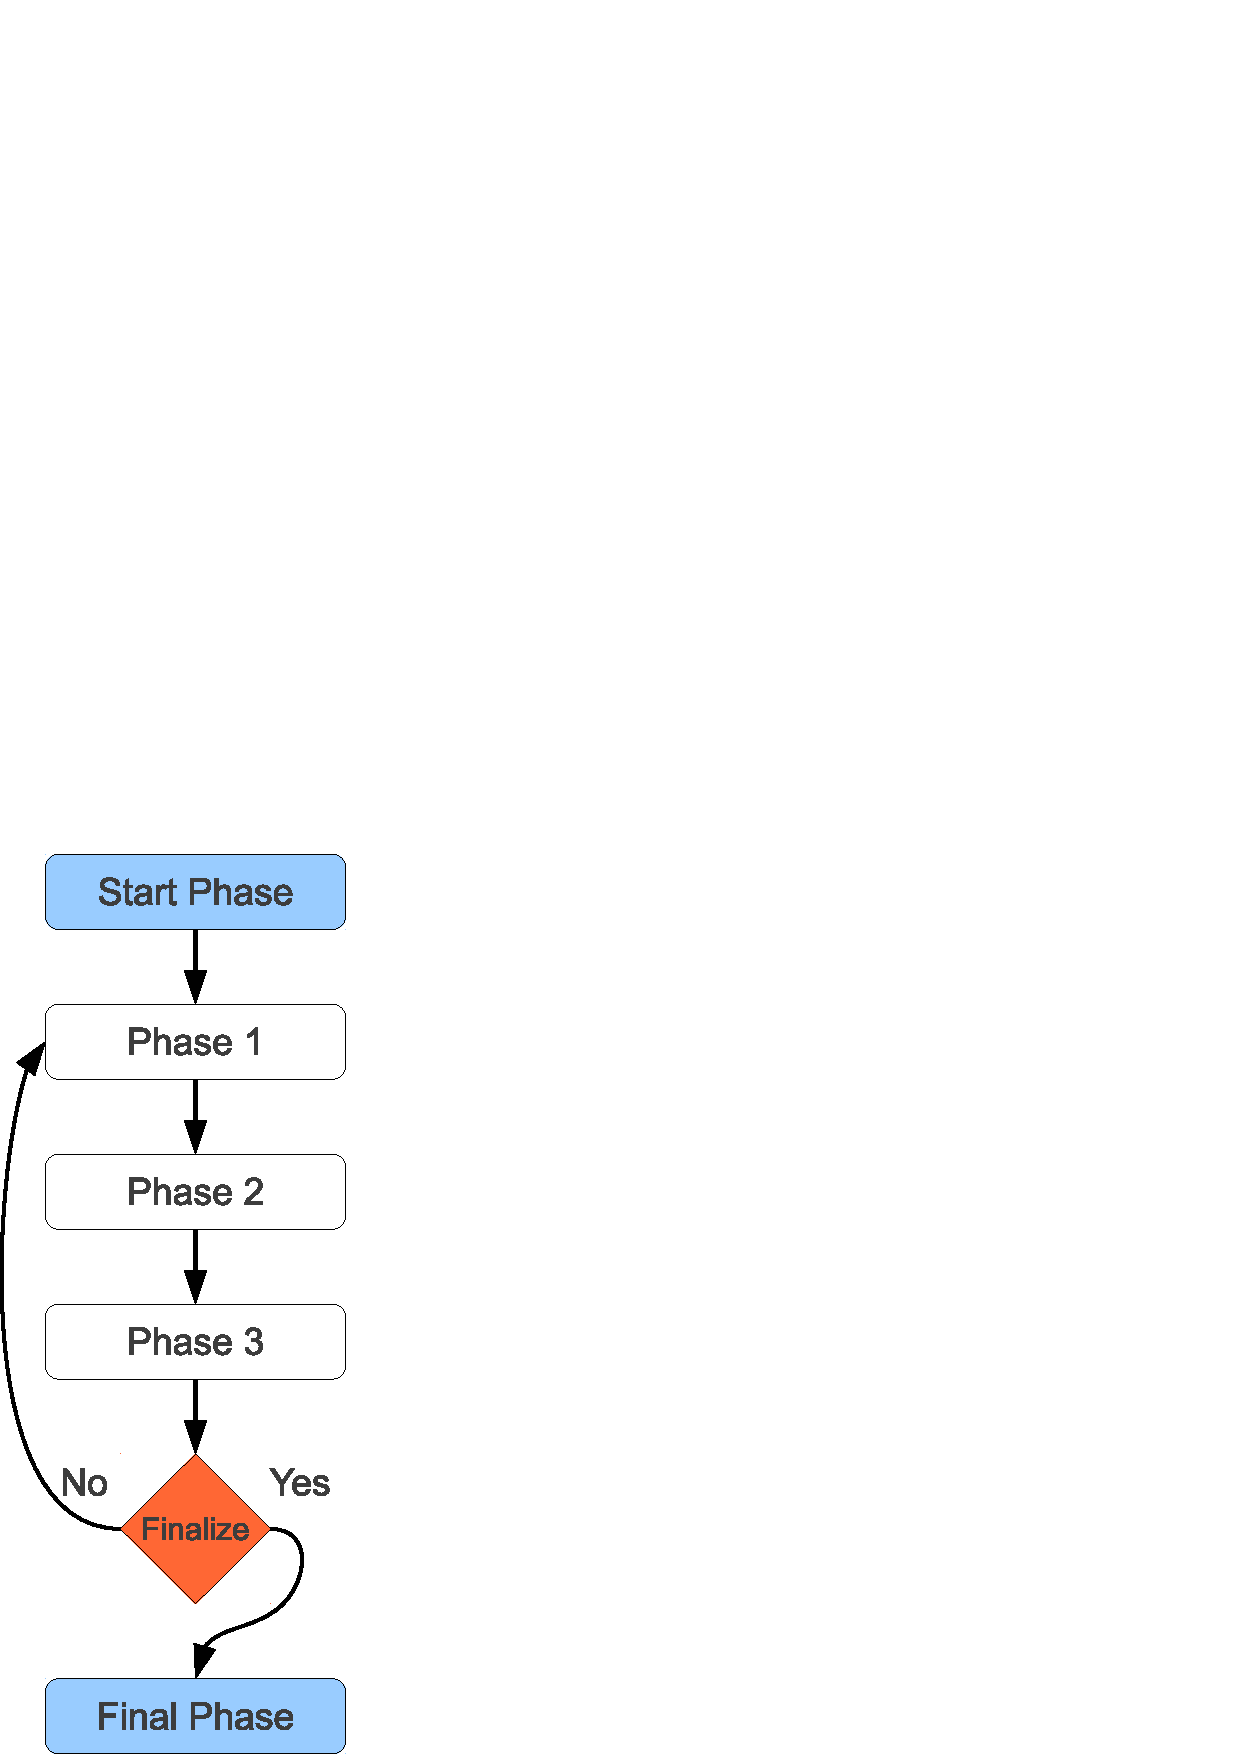
\includegraphics[width=0.2\textwidth]{Chapter3/figures/MotionSequence.pdf}
  \caption{Phase Execution Sequence for a Typical XML-Based Motion.}
  \label{fig:PhaseSequence}
\end{figure}


Figure~\ref{fig:PhaseSequence} shows the execution sequence of an example motion file. In general, XML-based motions define cyclic phases to generate continuous movement. For example, the walking motion has three main phases which create a cycle. If the motion trigger has not changed at the end of the last phase (\texttt{Phase 3}), we have to continue with the execution of the first phase (\texttt{Phase 1}), not with the final one. If the motion trigger is different at the end of the last phase, then we proceed to the final phase to terminate the current motion, before starting the new one (if any). As we saw in the structure of every XML-based motion file, each phase lists a set of joint values. These values are in degrees. To generate motions for our agent we need to create a motion string, which encloses information about each joint's velocity. The velocity of a joint $i$ is computed as follows:
\[
JointVelocity_i = \cfrac{DesiredJointValue_i - CurrentJointValue_i}{CurrentPhaseDuration}
\]
The $CurrentJointValue_i$ is provided by the corresponding perceptor message. 
A velocity value is calculated for each joint involved in the motion and the final output of the motion controller is sent to the server. Note that zero velocity is set for every joint not included in the \texttt{effector} field of the current phase, so that these joints stop moving. 



\subsection{Text-Based Motion Files}
The text-based motion files we use have been adopted from the Webots simulator~\cite{Webots04} and they provide left and right turn motions. These text-based motion files have simpler structure than the XML-based motion files. By default, each pose lasts two simulation cycles (40ms). The structure of these motion files is shown below.
\begin{verbatim}
#WEBOTS_MOTION,V1.0
LHipYawPitch,LHipRoll,LHipPitch,LKneePitch,LAnklePitch,...
00:00:000,Pose1,0,-0.012,-0.525,1.05,-0.525,0.012,0,...
00:00:040,Pose2,0,-0.011,-0.525,1.05,-0.525,0.011,0,...
00:00:080,Pose3,0,-0.009,-0.525,1.05,-0.525,0.009,0,...
00:00:120,Pose4,0,-0.007,-0.525,1.05,-0.525,0.007,0,...
00:00:160,Pose5,0,-0.004,-0.525,1.05,-0.525,0.004,0,...
00:00:200,Pose6,0,0.001,-0.525,1.051,-0.525,-0.001,0,...
00:00:240,Pose7,0,0.006,-0.525,1.05,-0.525,-0.006,0,...
00:00:280,Pose8,0,0.012,-0.525,1.05,-0.525,-0.012,0,...
00:00:320,Pose9,0,0.024,-0.525,1.05,-0.525,-0.024,0,...
\end{verbatim}
Lines starting with \texttt{\#} are comments. The fist non-comment line must list  all joints involved in the defined movement using their names separated by commas. As an example, a walk motion requires only the joints from the leg kinematic chains. The remaining lines define one pose each. From left to right, each line contains the duration of the pose, the pose number, and the desired angle (in radians) for each joint in the same order they were given at the beginning. Note that, unlike the XML-based motion files, here the same joint set must be used throughout the entire motion. 


\subsection{Text-Based Motion Controller}
The motion controller for text-based motions is based on the same principle as the XML-based controller. The joint values in the motion files represent radians, so we have to convert these values into degrees before we proceed. Each pose nominally corresponds to two cycles, but we can make it last one or two or three cycles depending on the speed (faster, normal, slower) at which we want the motion to be executed. The text-based motion controller can be customized to perform these motions in different ways. The following parameters can be modified:
\begin{description}
	\item[Duration] The time between poses in simulation cycles. By default, $Duration=2$.
	\item[PoseStep] The step for advancing from pose to pose. By default, $PoseStep=1$, but we can subsample the motion with other values, e.g. for $PoseStep=2$, we execute pose1, pose3, pose5, ...
\end{description}
The desired velocity of each joint $i$ is computed by:
\[
JointVelocity_i = \cfrac {Desired Joint Value_i - Current Joint Value_i} {Duration \times CycleDuration}
\]
Again, the $CurrentJointValue_i$ is provided by the corresponding perceptor message.
A velocity value is calculated for each joint involved in the motion and the final output of the motion controller is sent to the server. 

\begin{figure}[t!]
\centering
  \includegraphics[width=0.8\textwidth]{Chapter3/figures/DynamicTurn.pdf}
  \caption{Dynamic Walk Leaning: Left Leaning, No Leaning, Right Leaning.}
  \label{fig:Lean}
\end{figure}

\subsection{Dynamic Motion Elements}
In contrast to the general idea of static motion files, we have tried to implement some dynamic features into our motions. There is no much room for improvement in static motions, but with these features we managed to achieve some nice results.
\begin{description}
	\item[Walk Leaning] The XML-based walk motion can be dynamically modified to lean to the right or to the left. This is accomplished by altering the joint values of the (left or right) HipPitch and AnkePitch joints in specific phases of the walk motion. In effect, these changes force the corresponding leg to perform a slightly smaller step compared to the nominal step size. The end effect is a smooth walk motion which leans slightly to the left or to the right, as shown in Figure~\ref{fig:Lean}, saving time from a full body turn motion.
	\item[Walk Slowdown] Its important for our agent to slowdown while stopping in order to maintain stability. The XML-based walk motion can be dynamically modified by scaling the phase durations in order to achieve such a slowdown. Increasing the phase durations dynamically by about 35\% yields a smooth approach to a stopping position. 
	\item[Turn Gain] The text-based turn motions can be dynamically modified using a gain value for scaling the resulting velocities in order to perform the motion in a smoother or rougher way. By default, this gain value is set to $1.0$, however slightly smaller or larger values can result in useful variations of the defined motion. By dynamically changing this value between $0.3$ and $1.0$, the agent is able to turn its body anywhere between 7 and 40 degrees, as shown in Figure~\ref{fig:Turn}.
\end{description} 




\begin{figure}[t!]
\centering
  \includegraphics[width=0.8\textwidth]{Chapter3/figures/DynamicTurn.pdf}
  \caption{Dynamic Turn Gain: Turn Degrees (y-axis) against Gain Factor (x-axis).}
  \label{fig:Turn}
\end{figure}


\section{Actions}
In this section, we describe the way agents affect and change their environment. In our approach, actions are split into groups in terms of their complexity and type.

\subsection{Basic Actions}
Basic actions combine perceptual information and motion files in simple ways to achieve something useful. These basic actions are:
 
\subsubsection*{Look Straight}
 Moves the head to its nominal position. Both head joints are set to $0$.

\subsubsection*{Scan} 
Moves the head to perform periodic panning and tilting. 
 
\subsubsection*{Pan Head} 
Moves the head to perform periodic panning at zero tilt.
 
\subsubsection*{Track Object} 
Moves the head to bring a particular object to the center of the field of view. This action is applicable only when the object being tracked is visible, but, even when the object is visible, it is limited by the head joint ranges. 
 
\subsubsection*{Track Moving Object} 
This action estimates the direction and the speed of a moving object using a small number of observations, obtained while performing the Track Object action. It records a set of five consecutive observations and another set of five consecutive observations delayed by a fixed time period (the default is 5 cycles).  The difference between the average positions of each set gives a vector that reveals the direction of motion. Taking the ratio of the magnitude of this vector and the time delay yields the speed of the moving object. This action is applicable only when the moving object being tracked is visible, but, even when the object is visible, it is limited by the head joint ranges.
 
\subsubsection*{Find Opponent's Goals} 
This action finds the direction of the opponent's goal with respect to the agent by performing the Scan action until the opponent's goal becomes visible.

\subsubsection*{Look For Ball} 
Turns the body of the agent, while performing the Scan action, until the ball appears within the field of view.
 
\subsubsection*{Turn To Ball} 
Turns the body of the agent towards the direction of the ball, while performing the Track Ball action. It can applied only when a ball is visible.
 
\subsubsection*{Turn To Localize} 
Turns the body of the agent, while performing the Pan Head action, until the agent's belief about its own location is updated with confidence. It can be used when the agent needs to (re)localize itself into the field.

\subsubsection*{Stand Up} 
Makes the agent stand up on its feet, after a confirmed fall on the ground, whether face-up or face-down. This action monitors the inertial sensors (accelerometers and gyroscopes) to check if the agent has fallen on the ground. Incoming gyroscope and accelerometer values above a specific threshold indicate a possible fall, but this has to be confirmed, because it is not unusual to receive values above threshold due to collisions without a fall. To confirm a fall, the action checks the force resistance perceptors located under the agent's feet. If these perceptors indicate that the legs do not touch the ground, then we are quite sure that a fall has occurred. In this case, a stand up motion is executed. Foot pressure values are also used to determine whether the stand up motion succeeded or not. The stand up motion is repeated, until it succeeds. This action is applicable at all times, however a stand up motion is executed only when the robot lies on the ground. 

\begin{figure}[t!]
  \centering
  \includegraphics[trim=0cm 3cm 0cm 4cm, clip,width=0.6\textwidth]{Chapter3/figures/NaoKick.png}
  \caption{Nao Performing a Kick after Positioning for Kick.}
  \label{fig:NaoKick}
\end{figure}
  
\subsubsection*{Prepare for Kick} 
Positions the agent to an appropriate position with respect to the ball in order to perform a kick successfully. Only forward and side steps are used in this fine positioning. Figure~\ref{fig:NaoKick} shows an example of robot kicking a ball after completing this action.
  
\subsection{Complex Actions}
Complex actions combine perceptual information, motion files, and basic actions. They have a more complicated structure and aim to achieve specific goals. These complex actions are:





\subsubsection*{Avoid Obstacles} 
This action records all obstacles around the agent and derives an obstacle-free route to a specified target. Initially, this action stores the positions of all obstacles located within 2m from the agent by performing the Pan Head action and watching the perceptor messages. Due to the fact that the simulated Nao's head can pan from $-120^{\circ}$ to $+120^{\circ}$ and the field of view is $120^{\circ}$, we can obtain a complete imaging of all obstacles located close to our agent. It is common to observe the same obstacle more than once; in this situation we only store the average of these observations. In a dynamic, multi-agent environment it is important to avoid collisions with other agents or fixed landmarks, such as goal posts in our simulated soccer games. To avoid obstacles we rely on a simple, yet reliable and effective, method. For each recorded obstacle, we calculate two escape angles that determine the two directions (relative to the agent), which guarantee avoidance of the obstacle at a safe distance. All other angles between these two escape angles are considered to be forbidden. Afterwards, any escape angle of some obstacle that falls within the forbidden area of some other obstacle is discarded.  The precise calculation of the escape angle set is described in Algorithm~\ref{AngleSet}. The remaining escape angles, and particularly the escape way points they define (the points closest to the obstacle along the direction of the escape angles), are evaluated in terms of the angle and distance overhead they incur with respect to the agent orientation (for the angle) and the target (for the distance). The way point that minimizes the total overhead is selected as a temporary target for avoiding the obstacles, while making progress towards the target. This method yields dynamically consistent results, meaning that the temporary target does not change in subsequent cycles as long as the obstacles remain stationary, until they are cleared on the way to the real target. Obstacle avoidance is demonstrated in Figure~\ref{fig:ObstacleAvoidance}, in a simple scenario, where there are two obstacles between the agent and its target position. Two of the escape angles are discarded; the way point on the left is selected as a temporary target to clear the obstacles. 
 

\begin{algorithm}[t!]
\caption{Escape Angle Set Calculation}
\label{AngleSet}
\begin{algorithmic}[1]
\STATE {\bf Input: }$Obstacles = \lbrace O_{1},O_{2},...,O_{n} \rbrace $
\STATE {\bf Output: }$EscapeAngleSet$
\STATE
\FOR{$i = 1 \textbf{ to } n$}
\STATE find $LeftEscapeAngle_i$ for obstacle $O_i$
\STATE find $RightEscapeAngle_i$ for obstacle $O_i$
\ENDFOR
\STATE $EscapeAngleSet = \emptyset$
\FOR{$i = 1 \textbf{ to } n$}
\IF{$LeftEscapeAngle_i \not\in [LeftEscapeAngle_j,RightEscapeAngle_j], \forall  j\neq i$}
\STATE $EscapeAngleSet = EscapeAngleSet \cup \{LeftEscapeAngle_i\}$
\ENDIF
\IF{$RightEscapeAngle_i \not\in [LeftEscapeAngle_j,RightEscapeAngle_j], \forall  j\neq i$}
\STATE $EscapeAngleSet = EscapeAngleSet \cup \{RightEscapeAngle_i\}$
\ENDIF
\ENDFOR
\RETURN $EscapeAngleSet$
\end{algorithmic}
\end{algorithm}



 \begin{figure}[t!]
  \centering
  \includegraphics[width=0.6\textwidth]{Chapter3/figures/ObstacleAvoidance.pdf}
  \caption{Obstacle Avoidance.}
  \label{fig:ObstacleAvoidance}
\end{figure} 


\subsubsection*{Walk to Ball}
Makes the agent walk towards the ball and stop when the ball is close enough to perform a kick. First, it performs the Turn to Ball action and then walk towards the ball, slowing down when it comes close to the ball. Recall that the ball distance returned by the vision perceptor is the distance between the camera, which is attached to agent's head, and the ball, which lies on the ground. However, for approaching the ball with precision, we need the distance on the ground between the agent's feet and the ball. To compute this distance, we first use forward kinematics along the sagittal plane of the robot to derive the current height of the camera. Taking the agent's ankle as the origin, it is easy to calculate every joint's position from ankle to head in the two-dimensional space of the sagittal plane using only the current values of the AnklePitch, KneePitch, HipPitch joints. Having the ball distance and the height of the camera, the ground distance can be easily derived using the Pythagorean Theorem. 
\[
GroundDistance = \sqrt{BallDistance^2 + CameraHeight^2}
\]
Figure~\ref{fig:2dkinematics} explains the derivation of the ground distance to the ball.
 
 \begin{figure}[t!]
\centering
  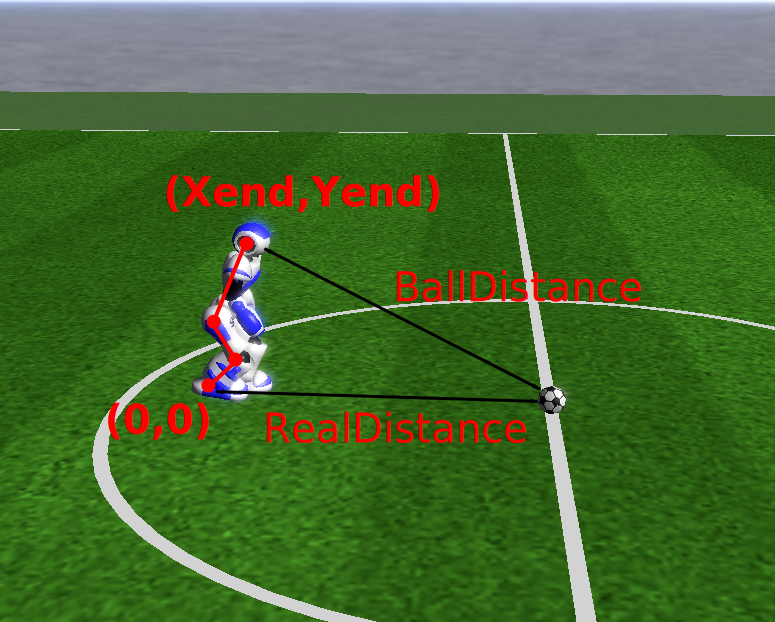
\includegraphics[trim=0cm 4cm 3cm 4cm,clip,width=0.8\textwidth]   {Chapter3/figures/2dkinematics.pdf}
  \caption{Ground Distance between the Agent and the Ball.}
  \label{fig:2dkinematics}
\end{figure}


\subsubsection*{On Ball Action} This action moves the agent close to the ball and executes an appropriate kick depending on the current state of the game. This action has a finite state machine logic shown in Figure~\ref{fig:GoKickBallToGoal}. It first performs the Walk To Ball action in order to reach the ball. After the successful completion of the Walk To Ball action, the agent performs the Find Opponent's Goal action. Subsequently, it aligns itself with the direction of the opponent's goal; the precision of this alignment is inversely proportional to the distance from the opponent's goal, meaning that far away from the opponent's goal there is more tolerance, since we only want to clear the ball from our own half of the field. Afterwards, it performs the Position for Kick action and finally it executes a kick motion. At any point of time, it is possible that an opponent agent takes the ball away from our agent; if that happens, the agent returns to the beginning.


 \begin{figure}[t!]
\centering
  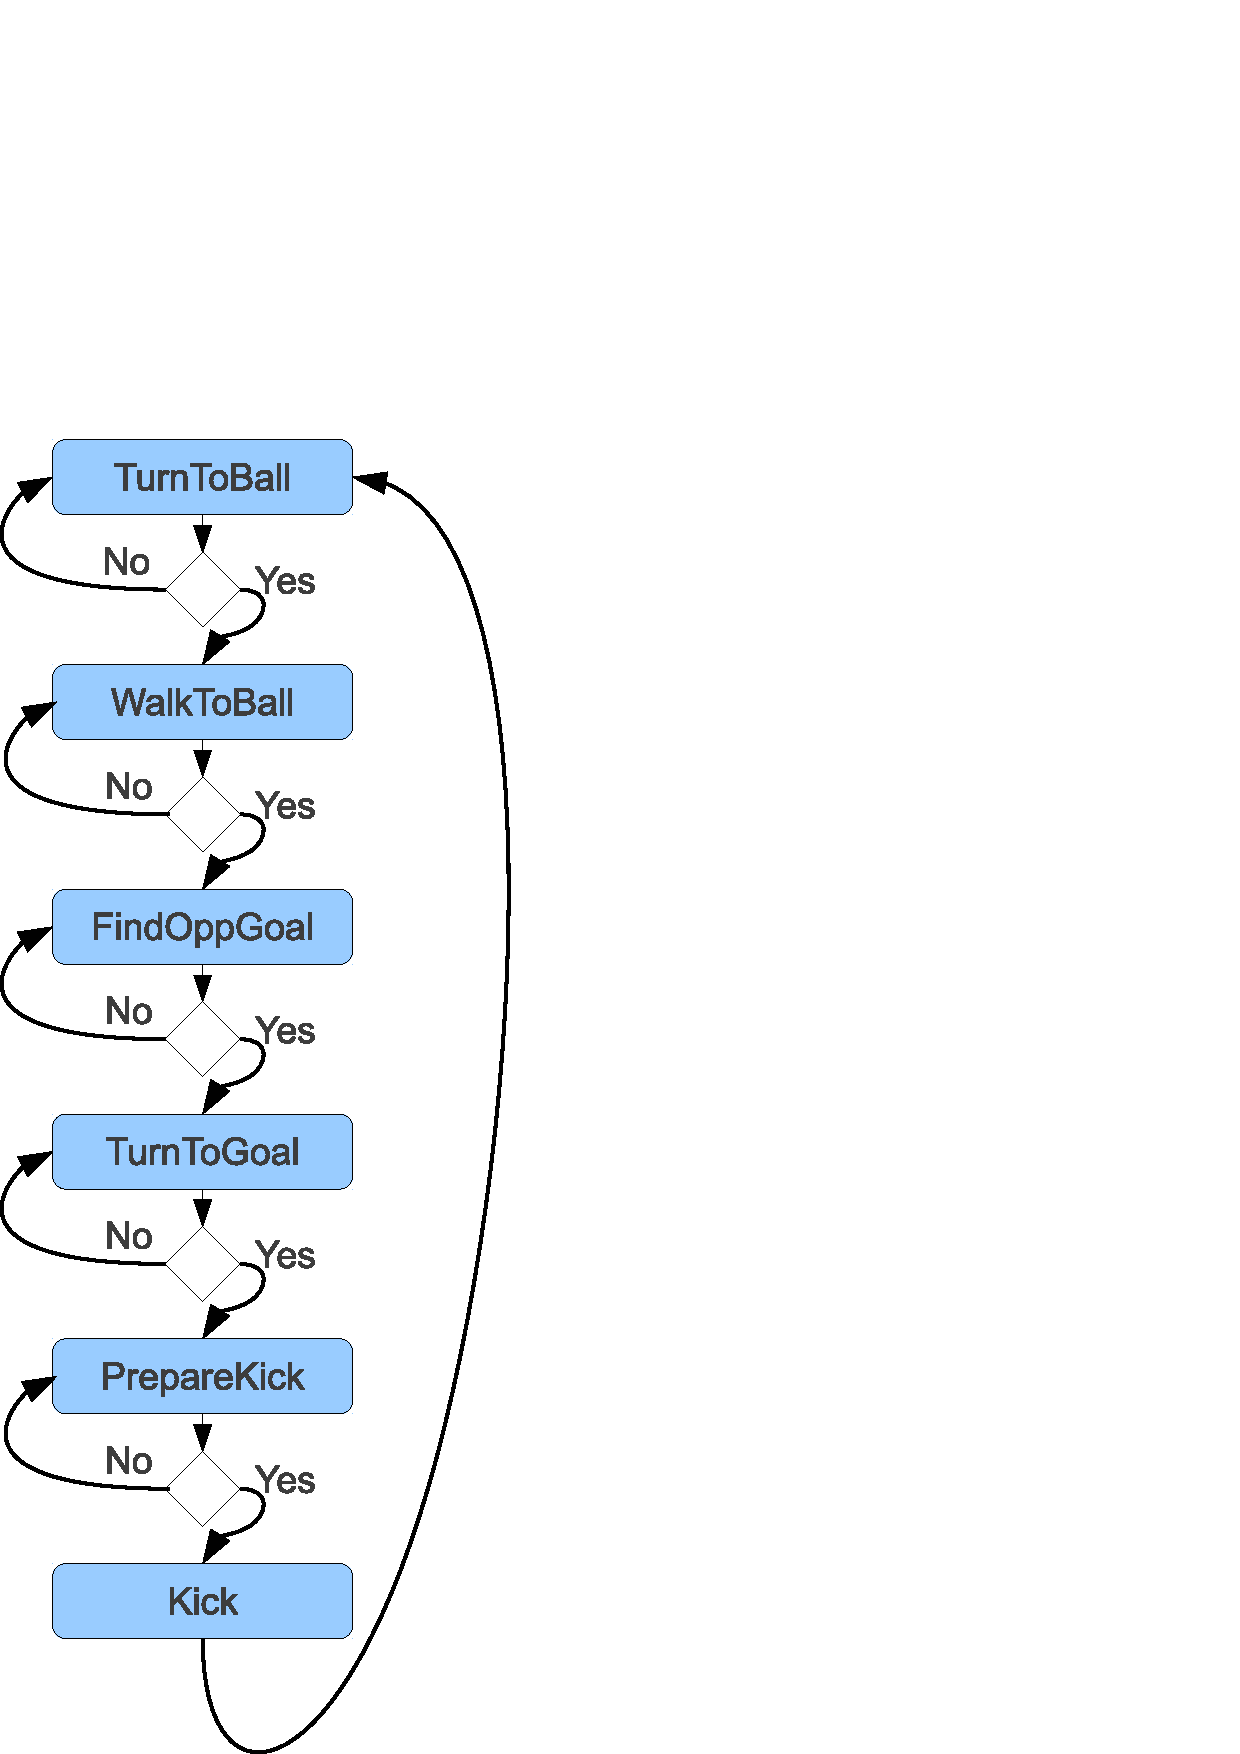
\includegraphics[width=0.25\textwidth]{Chapter3/figures/KickFSM.pdf}
  \caption{On Ball Action Logic Flowchart.}
  \label{fig:GoKickBallToGoal}
\end{figure}



\subsubsection*{Walk to Coordinate}
This action moves the agent to a specific location $(x_t, y_t, \theta_t)$ in the field. To perform this action we need to know our own location $(x_a, y_a, \theta_a)$ in the field; from there it is easy to calculate in which direction $\phi$ and at what distance $d$ to walk in order to reach the given target:
\begin{align*}
\phi &= \text{atan2}(x_t-x_a,y_t-y_a)\\
d &= \sqrt{(x_t-x_a)^2 + (y_t-y_a)^2}
\end{align*}
Figure~\ref{fig:WalkToCoordinate} shows an example of this calculation. The actual locomotion of the agent towards the target is done through the Avoid Obstacles action, which takes the pair $(d,\phi)$ as input and ensures that obstacles are avoided on the way to the target. Note that distance and direction are recalculated as the agent makes progress toward its target. After the position $(x_t,y_t)$ has been reached, a final rotation in place turns the agent towards the desired direction $\theta_t$. The action terminates when the agent reaches the desired location $(x_t, y_t, \theta_t)$.


 \begin{figure}[t!]
\centering
  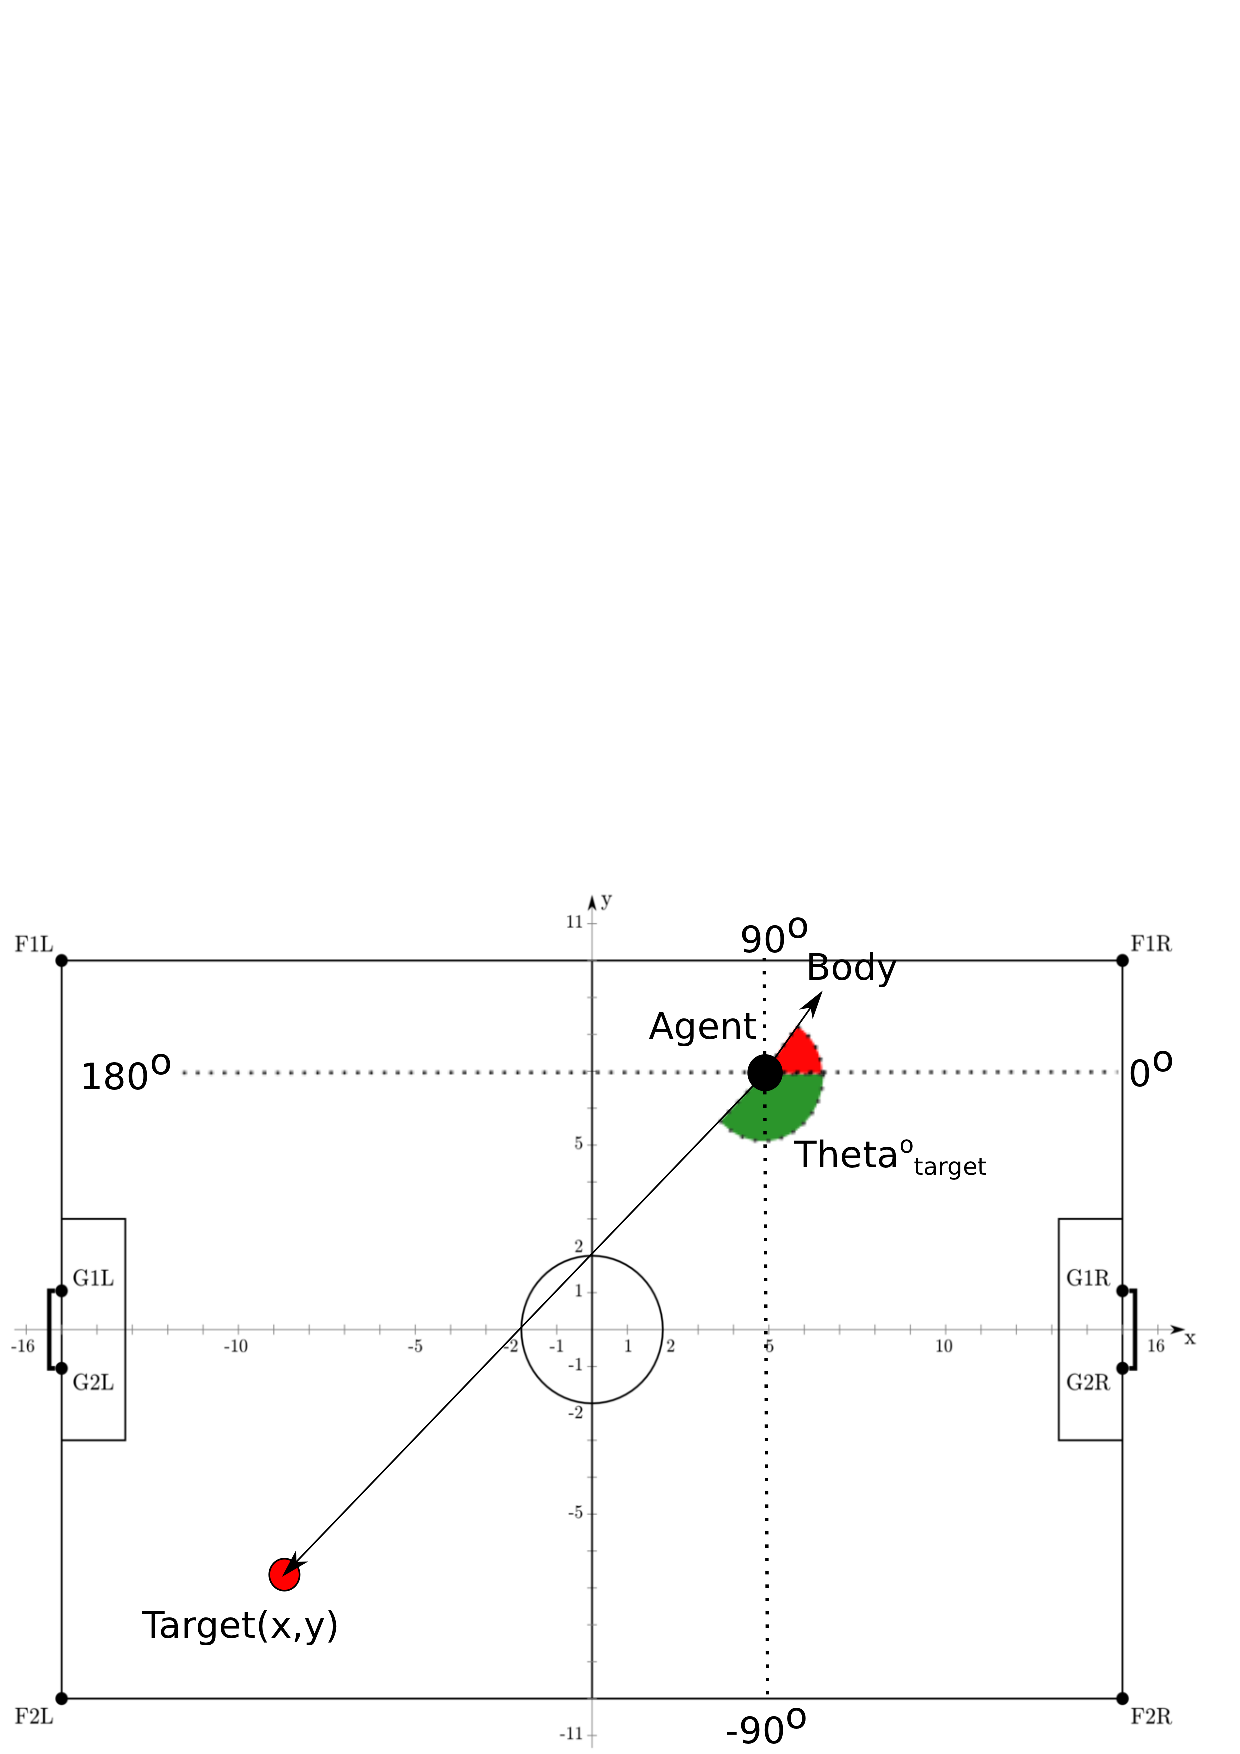
\includegraphics[width=0.8\textwidth]{Chapter3/figures/GoToPos.pdf}
  \caption{Walk To Coordinate Action.}
  \label{fig:WalkToCoordinate}
\end{figure}


\subsubsection*{Walk To Direction}
This action makes the agent walk towards a specific direction. First, it employs a turn in-place action to align with the given direction and then a straight walk action to move along the given direction. This action is not terminated by itself but there has to be a new action request or an ``empty'' action request. The actual locomotion of the agent towards the target direction is done through the Avoid Obstacles action.
 
\subsubsection*{Dribble Ball To Direction}
This action attempts to dribble the ball towards a specific direction. It is quite similar to the Walk To Direction action, however the agent  tries to keep the ball in front of its feet at all times.  The actual locomotion of the agent towards the target direction is done through the Avoid Obstacles action. This action is not fully functional in our software, since movements based on motion files make it hard to keep ball consistently in front of the agent. 



\section{Communication}
Communication in Simspark is not ideal. There are no restrictions about the use of the say effector and every agent can use it at each cycle. However, the hear perceptor comes with some restrictions (cf. Section~\ref{sec:soccerperceptors}). Messages shouted from beyond a maximum distance (currently 50 meters) cannot be heard. Given that the dimensions of the field are currently only $21m\times14m$ (version 0.6.5) or $20m\times 30m$ (version 0.6.6) (about $25m$ or $36m$ in diagonal length), there is no limit in practice. However, due to the limited communication bandwidth, we utilize the communication channel in the following way, to ensure that every message sent from an agent will be heard by the other agents in time. A simple communication protocol has been created in which time is sliced into pieces lasting one server cycle (20ms) each and repeats every three cycles (60ms). Figure~\ref{fig:TimeSlicing} shows how exactly time is sliced. The first of these three cycles is used for sending and the next two cycles are left idle on purpose to ensure that the message sent in the first cycle is delivered to all teammates. During the sending cycle, only one agent is allowed to send its message to the others. Every time slice of the protocol has an associated integer label which indicates the uniform number of the player able to send its message at that slice. This label starts at $1$ and grows by $1$ every time a player sends a message, until it reaches the maximum uniform number and loops back to number $1$. Since there is no common clock, to ensure that the agents are synchronized we make use of the changing game states, which are shared and known to all players; whenever the game state changes, the agents reset their integer label counters. Through this simple protocol, every player can receive reliably the messages from all teammates every 540ms (27 cycles) for a team of 9 players or every 660ms (33 cycles) for a team of 11 players.

\begin{figure}[t!]
\centering
  \includegraphics[width=0.8\textwidth]{Chapter3/figures/MAC.pdf}  
  \caption{Time Slicing Communication Protocol.}
  \label{fig:TimeSlicing}
\end{figure} 